\documentclass[uplatex,dvipdfmx,a4paper,twocolumn,base=11pt,jbase=11pt,ja=standard]{bxjsarticle}

\usepackage{ipsj}
\usepackage{color}
\usepackage{amssymb}

\title{チャネリング制約を用いた alldifferent 制約の SAT 符号化}{SAT Encoding of alldifferent Constraints with Channeling Constraints}
\author{名古屋大学}{小菅 脩司}{Shuji Kosuge, Nagoya University}
\author{神戸大学}{宋 剛秀}{Takehide Soh, Kobe University}
\author{神戸大学}{田村 直之}{Naoyuki Tamura, Kobe University}
\author{名古屋大学}{番原 睦則}{Mutsunori Banbara, Nagoya University}
\begin{document}
\maketitle

%%%%%%%%%%%%%%%%%%%%%%%%%%%%%%%%%%%%%%%%%%%%%%%%%%%%%%%%%% 
\chapter{緒論}

\pagenumbering{arabic}

\textbf{時間割問題} (Timetabling Problem) は,
求解困難な組合せ最適化問題の一種である.
この問題には,ハード制約とソフト制約が存在し,ソフト制約に違反するとペ
ナルティが与えられる.必ず満たすべきハード制約を満たしながら,ペナルティ
の総和を最小にするような解を求めることが目的である.
現状では,質の高い時間割を編成するために多くの人間の労力が費やされている.
このような背景から,時間割に関する国際会議
(Practice and Theory of Automated Timetabling; PATAT)
や国際時間割競技会 (International Timetabling Competition; ITC)
が開催され,時間割ソルバーの性能向上に貢献している.

\textbf{解集合プログラミング} (Answer Set Programming; ASP) 
\cite{%
  Baral03:cambridge,%
  Gelfond88:iclp,%
  Inoue08:jssst,%
  Niemela99:amai}
  は,
論理プログラミングから派生した宣言的プログラミングパラダイムの一つである.
ASP 言語は一階論理に基づく知識表現言語の一種であり,論理プログラムは
ASP のルールの有限集合である.ASP システムは論理プログラムから安定モデ
ル意味論に基づく解集合を計算するシステムである.
近年,SAT 技術を応用した高速 ASP システムが実現され,ロボット工学,シ
ステム生物学,システム検証,プランニングなど様々な分野への実用的応用が
急速に拡大している.

近年,\textbf{カリキュラムベース・コース時間割}
(Curriculum-based Course Timetabling; CB-CTT)
問題に対する ASP を用いた解法が提案され,成功を収めている
\cite{%
 banbara17:ramp}.
CB-CTT 問題は,大学等の1週間の講義スケジュールを求める問題であり,
最も研究が盛んな教育時間割問題の一つである.
ASP は系統的探索であることを活かして,未解決問題の最適値を決定するなど
優れた性能を示している.
しかし,その一方で,ソフト制約が多く含まれるような問題集において,
局所的探索を用いた解法より性能が劣っている場合が見られる.

この問題を解決するために,系統的探索と局所的探索を組み合わせた
\textbf{Large Neighborhood Prioritized Search} (LNPS)
\cite{%
 hayama19:kobe}
が提案されている.
LNPS は,暫定解に含まれる変数の値割り当ての一部をランダムに選んで取り
消し,他の値割り当てをなるべく維持したままで解を再構築する反復法の一種
である.
ASP を用いた LNPS の利点は,解の再構築を系統的探索で行え,値割り当てを
なるべく維持したままでの再構築が自然に実現できることである.
LNPS の性能は,
暫定解の一部をランダムに選んで取り消す destroy 演算子に依存するが,
十分な研究がなされてない.

本論文では,LNPS を用いたカリキュラムベース・コース時間割 (CB-CTT)
問題の解法について述べる.
CB-CTT に対する既存研究
\cite{%
 kiefer16:patat}
 を応用して,
3種類の destroy 演算子 (random, day-period, day-room) を実装した.
random が問題の性質をまったく利用しないのに対し,
day-period と day-room は CB-CTT のソフト制約を考慮して
暫定解の一部をランダムに選んで取り消す点が特長である.
%
提案手法の有効性を評価するために,国際時間割競技会 ITC-2007 のベンチマー
ク問題(21問)を用いて実行実験を行った.その結果,
多くの問題に対して,day-period と day-room が既存 ASP 解法より良い解を
生成し,提案手法の有効性が確認できた.

以降の構成は以下の通りである.
第二章で時間割問題,特に本論文が対象とするカリキュラムベース・コース時
間割問題について述べる.
第三章で解集合プログラミングについて述べ,その中で,LNPS の実装におい
て重要な変数選択ヒューリスティクスの変更機能について述べる.
第四章で LNPS 及び 実装した destroy 演算について述べる.
第五章でカリキュラムベース・コース時間割問題に実装解法を適用した実験の
結果を述べ,既存 ASP との比較や,destroy 演算同士での比較を交え考察を
行う.
最後に第六章で結論を述べる.

%%%%%%%%%%%%%%%%%%%%%%%%%%%%%%%%%%%%%%%%%%%%%%%%%%%%%%%%%% 


%%% Local Variables:
%%% mode: latex
%%% TeX-master: "paper"
%%% End:

% \chapter{alldifferent 制約の SAT 符号化}
\section{alldifferent 制約の SAT 符号化}

alldifferent 制約は alldifferent($x_1,\dots,x_n$) で表され,その要素$x_i$が互いに異なることを表す.
% この制約は
% $$\bigwedge_{1 \leq i < j \leq n} x_i \neq x_j$$
% を意味する.

直接符号化は各整数変数$x$とそのドメイン$a$について$x=a$であることを命題変数$p(x=a)$で表す.
$x$がそのドメイン$\{\ell,\ell+1,\dots,u\}$の中から少なくとも1つの値を取る制約を
$$p(x=\ell) \lor p(x=\ell+1) \lor \dots \lor p(x=u)$$
と表す.
$x$がそのドメイン$\{\ell,\ell+1,\dots,u\}$の中から多くとも1つの値を取る制約を
$$\lnot p(x=i) \land \lnot p(x=j) \;\; (\ell \leq i < j \leq u)$$
と表す.

順序符号化は各整数変数$x$とそのドメイン$a$について$x \leq a$であることを命題変数$p(x\leq a)$で表す.
$x$とそのドメイン$\{\ell,\ell+1,\dots,u\}$に対し,$p(x \leq \ell),p(x \leq \ell+1),\dots,p(x \leq u-1)$を導入し,その関係を
$$\lnot p(x \leq i) \lor p(x \leq i+1) \; (\ell \leq i \leq u-2)$$
と表す.


alldifferent$(x_1,\dots,x_n)$について$x_i\in \{ \ell,\ell+1,\dots,u \}$である時,
この制約は
$$\bigwedge_{1 \leq i < j \leq n} x_i \neq x_j$$
を意味する.
また,$x \neq x'$は
$$
\bigwedge_{\ell \leq a \leq u} (x \neq a \lor x' \neq a)
$$
で表すことができる.
直接符号化において,$x \neq a$は$\lnot p(x=a)$と符号化できる.
順序符号化において,$x \neq a$は$p(x \leq a-1) \lor \lnot p(x \leq a)$と符号化できる.


% alldifferent$(x_1,\dots,x_n)$について$x_i\in \{ \ell,\ell+1,\dots,u \}$である時,
% 直接符号化では
% $$\bigwedge_{1 \leq i < j \leq n} (p(x_i=a) \lor p(x_j=a)) \;\; (\ell \leq a \leq u)$$
% と符号化できる.
% 順序符号化では
% $$\bigwedge_{1 \leq i < j \leq n} (p(x_i \leq a-1) \lor \lnot p(x_i \leq a) \lor p(x_j \leq a-1) \lor \lnot p(x_j \leq a)) \;\; (\ell \leq a \leq u-2)$$
% と符号化できる.


%%% Local Variables:
%%% mode: latex
%%% TeX-master: "paper"
%%% End:

% \chapter{チャネリング制約を用いた alldifferent 制約の SAT 符号化}
\section{チャネリング制約を用いた alldifferent 制約の SAT 符号化}

順序符号化と直接符号化を組み合わせる際に用いた制約は以下の通りである.
$$p(x=a) \Leftrightarrow p(x \leq a) \land \lnot p(x \leq a)$$

チャネリングさせることで
順序符号化で有効な鳩の巣原理を用いたヒント制約や,
直接符号化で有効なat-least-one制約を組み合わせることができる.
alldiferent制約はPB・大野\cite{Ono19:ai}の手法で表現することができる.


\begin{table}[]
    \caption{提案した符号化一覧}
    \label{table:model}
    % {\scriptsize  \begin{tabular}[c] {c|c|c|c|c|c|c|c|c}
   & 整数変数の & \multicolumn{4}{|c|}{alldifferent制約の分解} & PHP & ALT1 \\\cline{3-6}
   & 符号化法   & $\neq$分解 & PB & PB3 & PB4 & & &\\\hline\hline
  0     & OE                    & OE      &    &       &             &     &     & \\
  1     & OE                    & OE      &    &       &             & OE  &     & (Sugarと同じ)\\\hline
  2     & OE$\Leftrightarrow$DE & DE      &    &       &             &     &     & \\
  3     & OE$\Leftrightarrow$DE & DE      &    &       &             &     & DE  & [Gent+ '04]\\
  4     & OE$\Leftrightarrow$DE & DE      &    &       &             & OE  &     & \\
  5     & OE$\Leftrightarrow$DE & DE      &    &       &             & OE  & DE  & \\
  6     & OE$\Leftrightarrow$DE &         & OE &       &             &     &     & \\
  7     & OE$\Leftrightarrow$DE &         & OE &       &             & OE  &     & \\
  8     & OE$\Leftrightarrow$DE &         &    & OE    &             &     &     & \\
  9     & OE$\Leftrightarrow$DE &         &    & OE    &             & OE  &     & \\
  10    & OE$\Leftrightarrow$DE &         &    &       & OE          &     &     & \\
  11    & OE$\Leftrightarrow$DE &         &    &       & OE          & OE  &     &
 \end{tabular}
}
    {\tiny  \begin{tabular}[c] {|c|c|c|c|c|c|c|c|}\hline
  model & 整数変数の            & \multicolumn{4}{|c|}{alldifferent} & PHP & ALT1 \\\cline{3-6}
        & 符号化法              & $\neq$ & PB & 大野3 & 大野4       &     &      \\\hline
  0     & OE                    & OE      &    &       &             &     &      \\
  1     & OE                    & OE      &    &       &             & OE  &      \\
  2     & OE$\Leftrightarrow$DE & DE      &    &       &             &     &      \\
  3     & OE$\Leftrightarrow$DE & DE      &    &       &             &     & DE   \\
  4     & OE$\Leftrightarrow$DE & DE      &    &       &             & OE  &      \\
  5     & OE$\Leftrightarrow$DE & DE      &    &       &             & OE  & DE   \\
  6     & OE$\Leftrightarrow$DE &         & OE &       &             &     &      \\
  7     & OE$\Leftrightarrow$DE &         & OE &       &             & OE  &      \\
  8     & OE$\Leftrightarrow$DE &         &    & OE    &             &     &      \\
  9     & OE$\Leftrightarrow$DE &         &    & OE    &             & OE  &      \\
  10    & OE$\Leftrightarrow$DE &         &    &       & OE          &     &      \\
  11    & OE$\Leftrightarrow$DE &         &    &       & OE          & OE  &      \\\hline
 \end{tabular}
}
\end{table}
% % model.tex の説明
% 1列目は提案した符号化の番号を表している.
% 2列目は alldifferent 制約の符号化手法を表している.
% OE は順序符号化法で符号化することを表している.
% OE\textless=\textgreater DE は順序符号化法と直接符号化法をチャネリングさせて符号化する符号化することを表している.
% 3列目は alldifferent 制約の分解方法を表している.
% neq はnot-equal 制約に分解することを表している.
% PB はブール基数制約を用いて分解することを表している.
% 大野3・大野4は[大野,'19]の手法3・4を用いて分解することを表している.
% 4列目は 鳩の巣原理を用いたヒント制約の有無を表している.
% チェックマークを付けたモデルにヒント制約として追加している.
% 5列目は At-least-one 制約の有無を表している
% チェックマークを付けたモデルにヒント制約として追加している.

% model2.tex の説明
表\ref{table:model}は提案した alldifferent 制約のSAT符号化手法の一覧である.
1列目は提案した符号化の番号を,
2列目は 整数変数の符号化手法を表している.
OE は順序符号化法で符号化することを,
OE$\Leftrightarrow$ DE は順序符号化法と直接符号化法をチャネリングさせて符号化する符号化することを表している.
3列目は alldifferent 制約の分解方法を表している.
その中で$\neq$ はnot-equal 制約,
PB はブール基数制約,
大野3・大野4は[大野,'19]の手法3・4を用いて分解することを表している.
そして,どの分解方法を用いるのかと,それぞれの分解方法が直接符号化と順序符号化のどちらで符号化されるかをDEとOEで表している.
4・5列目は 鳩の巣原理を用いたヒント制約とat-least-one制約を直接符号化と順序符号化のどちらで符号化するのかとその有無を表している.




%%% Local Variables:
%%% mode: latex
%%% TeX-master: "paper"
%%% End:

\section{実行実験}\label{chap:exp}
%%%%%%%%%%%%%%%%%%%%%%%%%%%%%%
\begin{figure*}[t]
  \centering
  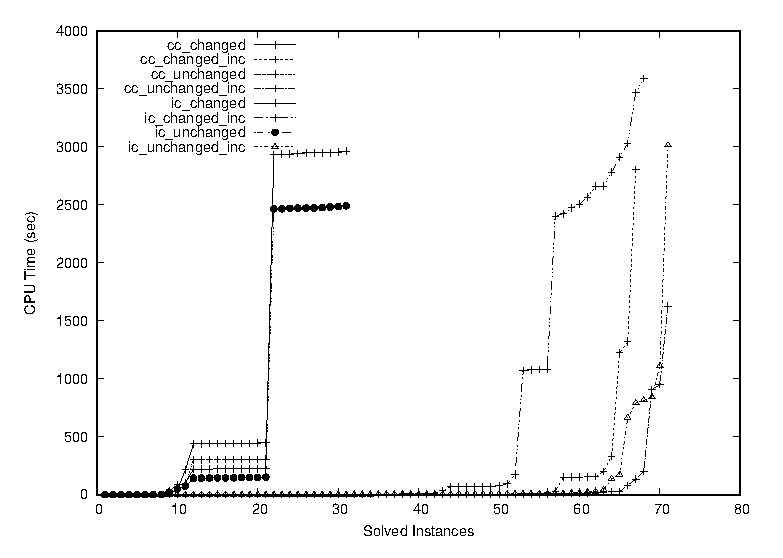
\includegraphics[scale=0.4]{fig/cactus.eps}
  \caption{基本符号化(コード~\ref{code:srf1.lp})と改良符号化(コード~\ref{code:srf2.lp})と
 発展符号化(コード~ \ref{code:srf3.lp})の比較} 
  \label{fig:cactus}
\end{figure*}
%%%%%%%%%%%%%%%%%%%%%%%%%%%%%%

%%%%%%%%%%%%%%%%%%%%%%%%%%%%%%
\begin{table*}[t]
  \caption{基本符号化(コード~\ref{code:srf1.lp})と改良符号化(コード~\ref{code:srf2.lp})と発展符号化(コード~ \ref{code:srf3.lp})の比較 (解けた問題数)} 
  \label{table:kibo}
  \centering
  \begin{tabular}[t]{rcr|c|ccc}
    \noalign{\hrule height 1pt}
    \multicolumn{3}{c|}{辺の数} & 問題数 & 基本符号化 & 改良符号化 & 発展符号化\\
    \noalign{\hrule height 1pt}
    %%%%%%%% 
       1 &~& 1000 & 30 & \textbf{30} & \textbf{30} & \textbf{30} \\ 
    1001 &~& 4000 & 20 & \textbf{20} & \textbf{20} & \textbf{20} \\ 
    4001 &~& 7000 & 11 & 9 & \textbf{10} & \textbf{10} \\ 
    7001 &~& 10000 & 8 & 4 & 6 & \textbf{8}  \\ 
    10001 &~& 20000 & 9 & 2 & 5 & \textbf{9} \\ 
    20001 &~& 30000 & 2 & 1 & \textbf{2} & \textbf{2} \\ 
    30001 &~& 40000 & 1 & 0 & 0 & \textbf{1} \\
    40001 &~& 50000 & 4 & 0 & 2 & \textbf{4} \\
    %%%%%%%% 合計
    \noalign{\hrule height 1pt}
    \multicolumn{3}{c|}{計} & 85 & 66 & 75 & \textbf{84} \\
    \noalign{\hrule height 1pt}
  \end{tabular}
\end{table*}
%%%%%%%%%%%%%%%%%%%%%%%%%%%%%%

%%%%%%%%%%%%%%%%%%%%%%%%%%%%%%
\begin{table*}[t]
  \centering
  \caption{配電網遷移問題のASP符号化(コード~\ref{code:pw-core})の実行結果}
  \label{table:core}
  \begin{tabular}{ccrrr}
 \rowcolor[RGB]{0,96,0}
\color{white}最短ステップ長 & \color{white}問題数 
     & \multicolumn{1}{c}{\color{white}シングルショット} 
         & \multicolumn{1}{c}{\color{white}マルチショット} 
             & \multicolumn{1}{c}{\color{white}シングル/マルチ} \\
 \rowcolor[RGB]{230,239,230}
1 & 6 & 1.677 & 1.035 & 1.620 \\
 \rowcolor[RGB]{196,230,196}
2 & 62 & 3.507 & 1.608 & 2.180 \\
 \rowcolor[RGB]{230,239,230}
3 & 189 & 6.089 & 2.155 & 2.826 \\
 \rowcolor[RGB]{196,230,196}
4 & 312 & 9.294 & 2.734 & 3.399 \\
 \rowcolor[RGB]{230,239,230}
5 & 280 & 13.338 & 3.361 & 3.968 \\
 \rowcolor[RGB]{196,230,196}
6 & 130 & 18.303 & 4.165 & 4.394 \\
 \rowcolor[RGB]{230,239,230}
7 & 21 & 24.483 & 5.086 & 4.814 \\
\noalign{\hrule height 0.5pt}
 \rowcolor[RGB]{196,230,196}
計 & 1000 & 76.691 & 20.114 & 3.807 \\
\end{tabular}


\end{table*}
%%%%%%%%%%%%%%%%%%%%%%%%%%%%%%

提案アプローチの有効性を評価するために,
節~\ref{chap:encode}と節~\ref{chap:core}の符号化に基づくソルバー
を開発し,実行実験を行った.

\textbf{根付き全域森問題.}
ベンチマークとしては,
DNET~\footnote{\url{https://github.com/takemaru/dnet}}
で公開されている配電網問題3問,および,
Graph Coloring and its Generalization~\footnote{\url{http://mat.tepper.cmu.edu/COLOR04/}}
で公開されているグラフ彩色問題をもとに生成した82問\footnote{%
グラフ彩色問題127問の中から,連結グラフで辺の数が50,000以下である
82問を使用した.根については全ノードの1/5をランダムに選んで使用した.
}を使用した.
ベンチマーク問題(計85問)の規模は,
ノード数11〜1406,辺の数16〜49629,根ノード数1〜281である.
%
ASPシステムには {\clingo}-5.4.0 (\textit{trendy})を使用し,
問題1問あたりの制限時間は1時間とした.
実験環境は,Mac mini,3.2 GHz Intel Core i7,64GB メモリである.

基本符号化と改良符号化と発展符号化の比較結果を
図~\ref{fig:cactus}に示す.
この図はカクタスプロットと呼ばれ,
縦軸がCPU時間,横軸が解けた問題数を表す.
グラフが下に寄るほどより高速に,右に寄るほどより多くの問題を解いたこと
を意味する.
図~\ref{fig:cactus}より,発展符号化は,他2つの符号化と比較して,より多く
の問題を高速に解いていることがわかる.

表~\ref{table:kibo}は,解けた問題数を,ベンチマーク問題に含まれる辺の数
で分類したものである.
発展符号化は,ほぼ全てのベンチマーク問題(85問中84問)が解けており,
大規模な問題に対する有効性が確認できた. 

\textbf{配電網遷移問題.}
ベンチマークとしては,DNETで公開されている実用規模の配電網問題
({\sf fukui-tepco},ノード数 432,根ノード数 72,電流上限 300)をベースにした.
この問題の実行可能解から,スタート状態を10個,ゴール状態を100個,
をランダムに選び,それらを組み合わせた計1000問の配電網遷移問題を生
成した.ASPシステムと実験環境は上と同じである.

配電網遷移問題のASP符号化(コード~\ref{code:pw-core.lp})の実行結果を
表~\ref{table:core}に示す.
左から順に,
問題名,
解を求めるまでのステップ長,解けた問題数,平均CPU時間を示している.
今回行った実行実験では,最長でステップ長が7の問題を解くことができた.


%%% Local Variables:
%%% mode: japanese-latex
%%% TeX-master: "paper"
%%% End:

%%%%%%%%%%%%%%%%%%%%%%%%%%%%%%%%%%%%%%%%%%%%%%%%%%%%%%%%%% 
\chapter{結論}
%%%%%%%%%%%%%%%%%%%%%%%%%%%%%%%%%%%%%%%%%%%%%%%%%%%%%%%%%%

XXX

%%% Local Variables:
%%% mode: latex
%%% TeX-master: "paper"
%%% End:


\end{document}
